\begin{figure}[h!]
\begin{center}
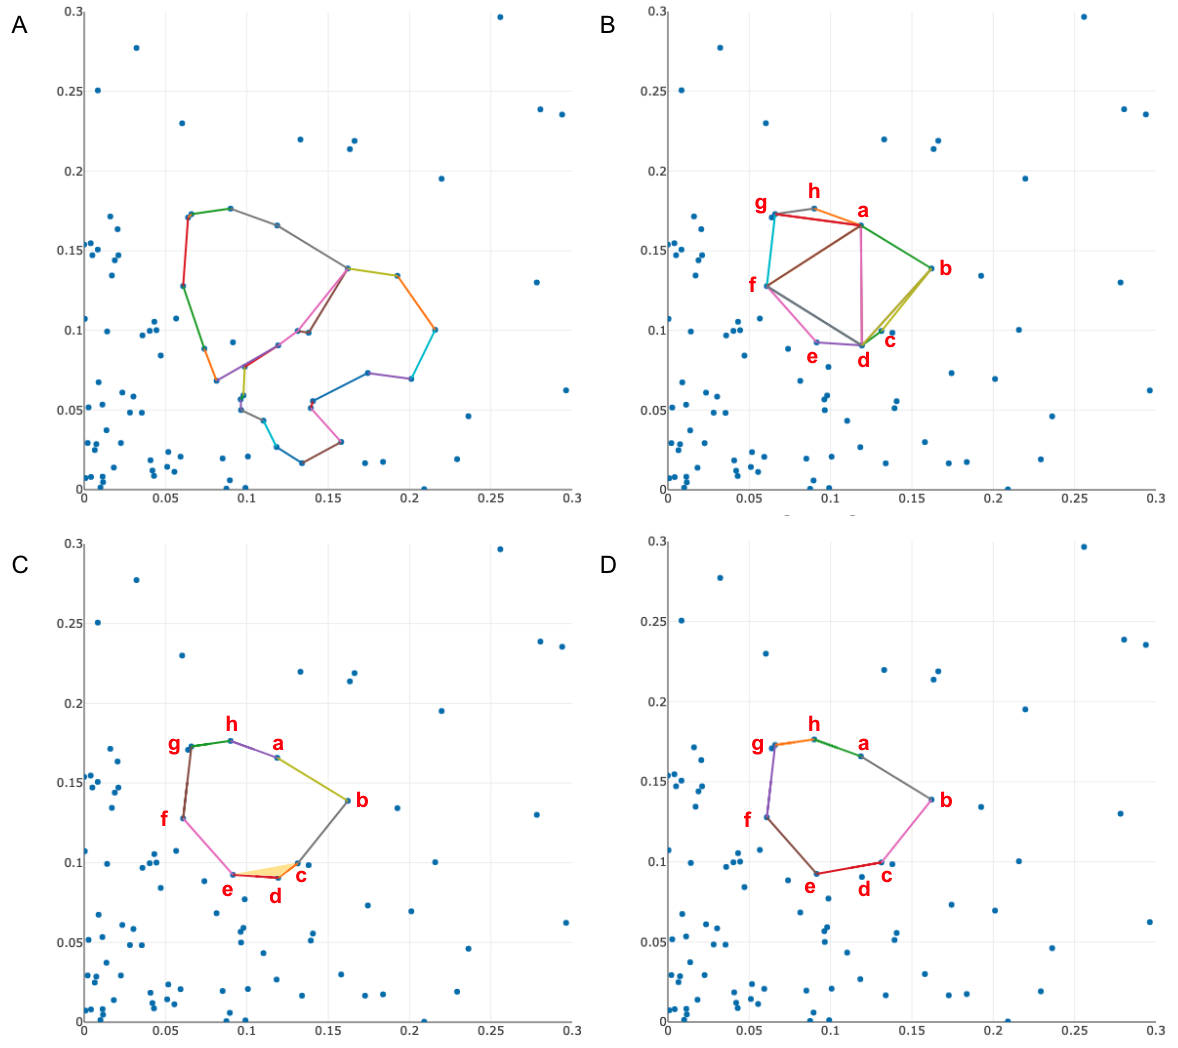
\includegraphics[width=15cm]{figures/areaExample4-2.png}
\end{center}
\caption{An example illustrating when the area enclosed by the triangle-loss area-weighted optimal cycle, solution to \pr \ref{itm:tri_NIA}, can be larger than the area enclosed by the edge-loss length-weighted minimal cycle, solution to \pr \ref{itm:edge_NIL}. \textbf{(A)} is the original cycle of a representative point cloud in $\mathbb{R}^2$ drawn from the normal distribution, \textbf{(B)} is the area-weighted optimal cycle triangulated based on the 2-simplices identified by nonzero entries in the coefficient vector $\volvec$, \textbf{(C)} is the area-weighted minimal cycle, \textbf{(D)} is the length-weighted minimal cycle. The yellow shaded area in \textbf{(C)} marks the difference in enclosed area by the area-weighted and length-weighted minimal cycle representatives. %The area-weighted volume optimal cycle contains the extra 2-simplex $[c,d,e].$
Constraint Equation \eqref{obacond1} specifies that the area-weighted optimal cycle must contain the 2-simplex born at the death time of the cycle. Therefore, this cycle must contain $\{a,d,f\}$ because it was born at the death time, and in fact, it contains both  $\{a,d,f\}$ and  $\{a,b,d\}$. The length-weighted minimal cycle does not have this constraint, and as such, can result in a smaller area. %\LL{Updated 0314}
%To get the length-weighted optimal cycle from the area-weighted volume optimal cycle, we still need to add the $2$-simplex $[c,d,e]$, which will increase the area-weighted volume, but will decrease the enclosed area. \LZ{I rephrased the previous sentence as: The length-weighted optimal cycle adds the $2$-simplex $[c,d,e]$ to the area-weighted volume optimal cycle, which increases the area-weighted volume but decreases the enclosed area....but now I don't think I understand the last part. The length-weighted does not care about the 2-simplices enclosed.}\CT{maybe: Our area-weighted volume optimal cycle differs from the length-weighted optimal cycle by the 2-simplex $[c,d,e]$. Although adding this 2-simplex would decrease the area of the cycle representative, it would increase our measured cost $||W\optimalrep||_1$.} 
}\label{fig:areaExample}
\end{figure}

